\documentclass[pra, onecolumn, notitlepage, floats, 11pt]{revtex4-1}

\usepackage[T1]{fontenc}
\usepackage{graphicx}
\usepackage{color}
\usepackage{latexsym,amsmath}
\usepackage{comment}
\usepackage{tabularx}
\usepackage{siunitx}
\usepackage{multirow}
\usepackage{mathtools}
\usepackage{tikz, fp}
\usepackage{wrapfig}
\usepackage{amsfonts}
\usepackage[pdftex,colorlinks=true, pdfstartview=FitV, linkcolor=linkcolor, citecolor=linkcolor, urlcolor=linkcolor, hyperindex=true,hyperfigures=true]{hyperref} %hyperlink%
\usepackage{fancyhdr}
\usepackage{inconsolata}
\usepackage{listings}
\usepackage{physics}
\usepackage{datetime}
\usepackage[caption=false]{subfig}
% \usepackage{subcaption}
% \usepackage{caption}
\usepackage{titlesec}

\renewcommand{\figurename}{Figure}
\renewcommand{\tablename}{Table}
\renewcommand{\thetable}{\arabic{table}}
% \renewcommand{\thefigure}{\textbf{\arabic{figure}}}
% \captionsetup{justification=justified,singlelinecheck=true}

\definecolor{airforceblue}{rgb}{0.36, 0.54, 0.66}  %#5D8AA8
\definecolor{cobalt}{rgb}{0.0, 0.28, 0.67}         %#0047AB
\definecolor{coolblack}{rgb}{0.0, 0.18, 0.39}      %#002E63
\definecolor{dartmouthgreen}{rgb}{0.05, 0.5, 0.06} %#00693E
\definecolor{lava}{rgb}{0.81, 0.06, 0.13}          %#CF1020
% move section headings to left
% \sffamily
% \scshape
%\titleformat{\section}{\raggedright\sffamily\bfseries\fontsize{13pt}{13}\selectfont}{\arabic{section}}{1em}{\MakeUppercase}
\titleformat{\section}{\raggedright\bfseries\scshape\fontsize{13pt}{13}\selectfont}{\color{cobalt}\arabic{section}}{1em}{\color{cobalt}}
\titleformat{\subsection}{\raggedright\bfseries\scshape\fontsize{12pt}{12}\selectfont}{{\color{cobalt}\arabic{section}.\arabic{subsection}}}{1em}{\color{cobalt}}
\renewcommand{\thesection}{\arabic{section}}
\renewcommand{\thesubsection}{\arabic{subsection}}
\renewcommand{\thesubsubsection}{\arabic{subsubsection}}
\makeatletter
\renewcommand{\p@subsection}{\thesection.}
\renewcommand{\p@subsubsection}{\thesection.\thesubsection.}
\makeatother


\linespread{0.956}

\DeclarePairedDelimiter\ceil{\lceil}{\rceil}
\DeclarePairedDelimiter\floor{\lfloor}{\rfloor}

\definecolor{linkcolor}{rgb}{0,0,0.65}
\definecolor{shadecolor}{rgb}{0.95, 0.95, 0.95}
\definecolor{mygreen}{rgb}{0,0.6,0}
\definecolor{mygray}{rgb}{0.5,0.5,0.5}
\definecolor{mymauve}{rgb}{0.58,0,0.82}
\lstdefinestyle{fortran}
{
    backgroundcolor=\color{shadecolor},       % background color
    basicstyle=\ttfamily\footnotesize,        % the size of the fonts that are used for the code
    breakatwhitespace=false,                  % sets if automatic breaks should only happen at whitespace
    breaklines=false,                         % sets automatic line breaking
    captionpos=b,                             % sets the caption-position to bottom
    commentstyle=\color{mygreen},             % comment style
    extendedchars=true,                       % lets you use non-ASCII characters; for 8-bits encodings only, does not work with UTF-8
    keepspaces=true,                          % keeps spaces in text, useful for keeping indentation of code (possibly needs columns=flexible)
    keywordstyle=\bfseries\color{blue},       % keyword style
    language=[95]Fortran,                     % the language of the code
    numbers=left,                             % where to put the line-numbers; possible values are (none, left, right)
    numbersep=5pt,                            % how far the line-numbers are from the code
    numberstyle=\tiny\color{mygray},          % the style that is used for the line-numbers
    rulecolor=\color{black},                  % if not set, the frame-color may be changed on line-breaks within not-black text (e.g. comments (green here))
    showspaces=false,                         % show spaces everywhere adding particular underscores; it overrides 'showstringspaces'
    showstringspaces=false,                   % underline spaces within strings only
    showtabs=false,                           % show tabs within strings adding particular underscores
    stepnumber=1,                             % the step between two line-numbers. If it's 1, each line will be numbered
    stringstyle=\color{mymauve},              % string literal style
    tabsize=4,                                % sets default tabsize to 4 spaces
    title=\lstname                            % show the filename of files
}

\lstdefinestyle{python}
{
    backgroundcolor=\color{shadecolor},       % background color
    basicstyle=\ttfamily\footnotesize,        % the size of the fonts that are used for the code
    breakatwhitespace=false,                  % sets if automatic breaks should only happen at whitespace
    breaklines=false,                         % sets automatic line breaking
    captionpos=b,                             % sets the caption-position to bottom
    commentstyle=\color{mygreen},             % comment style
    extendedchars=true,                       % lets you use non-ASCII characters; for 8-bits encodings only, does not work with UTF-8
    keepspaces=true,                          % keeps spaces in text, useful for keeping indentation of code (possibly needs columns=flexible)
    keywordstyle=\bfseries\color{blue},       % keyword style
    language=Python,                          % the language of the code
    numbers=left,                             % where to put the line-numbers; possible values are (none, left, right)
    numbersep=5pt,                            % how far the line-numbers are from the code
    numberstyle=\tiny\color{mygray},          % the style that is used for the line-numbers
    rulecolor=\color{black},                  % if not set, the frame-color may be changed on line-breaks within not-black text (e.g. comments (green here))
    showspaces=false,                         % show spaces everywhere adding particular underscores; it overrides 'showstringspaces'
    showstringspaces=false,                   % underline spaces within strings only
    showtabs=false,                           % show tabs within strings adding particular underscores
    stepnumber=1,                             % the step between two line-numbers. If it's 1, each line will be numbered
    stringstyle=\color{mymauve},              % string literal style
    tabsize=4,                                % sets default tabsize to 4 spaces
    title=\lstname                            % show the filename of files
}


\pagestyle{fancy}
\fancyhf{}
\fancyhead[L]{Rocco Ardino (Mat. 1231629)}
\fancyhead[R]{\bf\thepage}
\fancyfoot[L]{\textsc{report}: Week 4}
\fancyfoot[R]{\today}
\renewcommand{\headrulewidth}{0.1pt}
\renewcommand{\footrulewidth}{0.1pt}

\newcommand{\codebold}[2][cobalt]{\texttt{\bfseries {\color{#1}#2}}}
\newcommand{\code}[2][black]{\color{#1}\texttt{#2}}
\newcommand{\codefunctionbold}[2]{\texttt{\bfseries {\color{cobalt}#1}({\color{lava}#2})}}
\newcommand{\codefunction}[2]{\texttt{#1(#2})}










\begin{document}

\title{Quantum Information and Computing 2020/21\\Week 4 report}

\author{Rocco Ardino}

\date{\today}





\begin{abstract}
    Studying the performances of an algorithm, depending on some input variables, requires a certain level of automatization. This task can be easily accomplished using scripting languages such as Python. In this work, we take as algorithm the square matrices multiplication, whose CPU time consumption depends on the matrices size. The results are then stored, fitted and compared through meaningful plots with a model based on computational complexity considerations.
\end{abstract}

\maketitle


\section{Theory}
Let us consider two matrices \( A \in \mathbb{R}^{n \times m} \) and \( B \in \mathbb{R}^{p \times q} \), of dimensions respectively \( n \times m \) and \( p \times q \). If \( m = p \), it is possible to compute the matrix product \( AB \) and the result is a matrix \( C \in \mathbb{R}^{n \times q} \) of dimensions \( n \times q \), with matrix elements:
\begin{equation}
    c_{ij}
    =
    \sum_{k=1}^{p} a_{ik} b_{kj},
    \qquad
    ^{i=1,\dots,n}_{j=1,\dots,q}
    \quad .
    \label{eq:03_T_MATMUL}
\end{equation}
This algorithm is implemented in a very simple way through:
\begin{itemize}
    \item a loop over \( k \) for the calculation of a single matrix element (complexity: \( \mathcal{O}(m=p) \));
    \item two loops over \( i \) and \( j \) for the calculation of all the entries of the product matrix (complexity: \( \mathcal{O}(nq) \))
\end{itemize}
Therefore, the overall complexity of the operation is \( \mathcal{O}(nmq) \), being \( \mathcal{O}(n^3) \) for the special case of two square matrices multiplication.

From a mathematical point of view, the order of the three loops is irrelevant for the result. However, it affects the performances depending on the way a language stores variables in memory.





\section{Code Development}
The modules \codebold{matrixmod} and \codebold{err\_handling\_mod} from the previous weeks are employed in this work along with a Python script for automatization of the study. The code for matrix matrix multiplication implemented in Fortran is explained in Subsection \ref{ssec:04_C_SS_1}. The core functionalities of the Python script are explained in Subsection \ref{ssec:04_C_SS_2}.





\subsection{Matrix matrix multiplication algorithms}
\label{ssec:04_C_SS_1}
Matrix matrix multiplication algorithms have several possible implementations, depending on the order of the loops needed to access to the memory. For our study, we limit to two possible orders, corresponding to two user-defined functions:
\begin{itemize}
    \item \codefunctionbold{matmul\_col}{mat1,mat2}: the loop over consecutive elements of memory is the inner one. Its implementation is skectched in Listing \ref{lst:04_SS_2_1};
    \item \codefunctionbold{matmul\_row}{mat1,mat2}: the loop over consecutive elements of memory is the outer one. Its implementation is skectched in Listing \ref{lst:04_SS_2_2}.
\end{itemize}
Concerning their performances, the first method is expected to run faster since it exploits the rapid access to consecutive memory elements. However, the intrinsic Fortran implementation of \code{MATMUL} outperforms both the implementations, so all these three possibilities will be compared in the final results.

\medskip
\begin{lstlisting}[
    style=fortran,
    frame=single,
    label={lst:04_SS_2_1},
    caption={Implementation of the first algorithm of matrix matrix multiplication \code{matmul\_col}.}
]
function matmul_col(mat1, mat2) result(res)
    ...

    ! mat1 and mat2 dimensions
    N = size(mat1, 1)
    M = size(mat1, 2)
    P = size(mat2, 1)
    Q = size(mat2, 2)

    ! pre-conditions and debug checks:
    ! * if input matrices have valid dimensions
    ! * if input matrices are multiplicable
    ...

    ! loop for matrix matrix multiplication
    do jj=1,Q
        do kk=1,M
            do ii=1,N
                res(ii,jj) = res(ii,jj) + mat1(ii,kk)*mat2(kk,jj)
            end do
        end do
    end do
end function
\end{lstlisting}

\begin{lstlisting}[
    style=fortran,
    frame=single,
    label={lst:04_SS_2_2},
    caption={Implementation of the second algorithm of matrix matrix multiplication \code{matmul\_row}.}
]
function matmul_row(mat1, mat2) result(res)
    ...

    ! mat1 and mat2 dimensions
    N = size(mat1, 1)
    M = size(mat1, 2)
    P = size(mat2, 1)
    Q = size(mat2, 2)

    ! pre-conditions and debug checks:
    ! * if input matrices have valid dimensions
    ! * if input matrices are multiplicable
    ...

    ! loop for matrix matrix multiplication
    do ii=1,N
        do kk=1,M
            do jj=1,Q
                res(ii,jj) = res(ii,jj) + mat1(ii,kk)*mat2(kk,jj)
            end do
        end do
    end do
end function
\end{lstlisting}

The three functions \code{matmul\_col}, \code{matmul\_row} and \code{MATMUL} are called in a test program, which takes as input command-line argument an integer representing the dimension of two square matrices to multiply. The way the input argument is taken and handled is sketched in Listing \ref{lst:04_C_SS_1_3}. Then, the CPU time needed for the operation is computed for every implementation and printed on the standard output.

\medskip
\begin{lstlisting}[
    style=fortran,
    frame=single,
    label={lst:04_C_SS_1_3},
    caption={Handling of square matrix size \( n \) input argument.}
]
! square matrices dimension
integer(4) :: N

! get command-line arguments (square matrix size)
character(len=:), allocatable :: argument
integer*4 :: arglen
call GET_COMMAND_ARGUMENT(1, length=arglen)
allocate(character(arglen) :: argument)
call GET_COMMAND_ARGUMENT(1, value=argument)

! convert command line argument to integer (matrix size)
read(argument(:),'(i5)') N
\end{lstlisting}



\subsection{Python script for automatization}
\label{ssec:04_C_SS_2}
To test the performances of the three algorithms depending on the matrices size, it is convenient to run the Fortran executable from a Python script for different values of \( n \). For every run, the script takes the standard output with CPU time results and converts it to three numerical values, one for every algorithm. This trick is described in Listing \ref{lst:04_C_SS_2_1}.

\medskip
\begin{lstlisting}[
    style=python,
    frame=single,
    label={lst:04_C_SS_2_1},
    caption={Python function to convert standard output of Fortran executable to CPU time numerical values.}
]
import numpy as np
import os
import subprocess

# function for converting fortran output into numerical results
def get_output(cmd, N):
    results = subprocess.run([cmd, str(N)], stdout=subprocess.PIPE)
    results = results.stdout.decode('utf-8').strip().split('\n')
    results = [float(res.strip()) for res in results]
    return np.array(results)
\end{lstlisting}

Therefore, the script in order:
\begin{itemize}
    \item launches the Fortran executable \( m \) times for every single value of \( n \);
    \item gets the CPU time for each of the \( m \) samples;
    \item takes the mean value and the standard deviation over the \( m \) samples;
    \item does the previous steps for every algorithm and stores the respective results in .dat files.
\end{itemize}
These steps are described in Listing \ref{lst:04_C_SS_2_2}.

\medskip
\begin{lstlisting}[
    style=python,
    frame=single,
    label={lst:04_C_SS_2_2},
    caption={Sketch of code for scan on the square matrices size \( n \).}]
# No optimization flags
for j in range(len(Oflags)):
    Oflag = Oflags[j]
    print("["+Oflag+"] : start -------------------------------------------")
    os.system(comp + Oflag + opt + exec + src)
    for N,i in zip(Ns,range(len(Ns))):
        print("Running matmul functions for N = " + str(N))
        res = np.zeros((3,M))
        for k in range(M):
            res[:,k] = get_output(cmd, N)
        # store mean
        matmul_col_data[i,j] = np.mean(res[0,:])
        matmul_row_data[i,j] = np.mean(res[1,:])
        matmul_data[i,j]     = np.mean(res[2,:])
        # store standard deviation
        matmul_col_data[i,j+len(Oflags)] = np.std(res[0,:]) / np.sqrt(M)
        matmul_row_data[i,j+len(Oflags)] = np.std(res[1,:]) / np.sqrt(M)
        matmul_data[i,j+len(Oflags)]     = np.std(res[2,:]) / np.sqrt(M)
    print("["+Oflag+"] : end ---------------------------------------------")
\end{lstlisting}

Lastly, the output files are used to plot the results through a gnuplot script. Moreover, the ladder performs several fits for every dataset.





\section{Results}
The CPU time of the three algorithms under study is monitored for \( n \) spanning between \( N_{\mathrm{min}} = 50 \) and \( N_{\mathrm{max}} = 2000 \). In particular, \( 30 \) values of \( n \) are chosen in this interval using a log-spacing, since the plots of the results are showed in log-log scale. The number of samples \( m \) for the mean value and standard deviation computation is fixed to \( 5 \). So, the results without the use of optimization flags at compile time are displayed in Figure \ref{fig:04_R_1}.

\begin{figure}[!h]
	\centering
	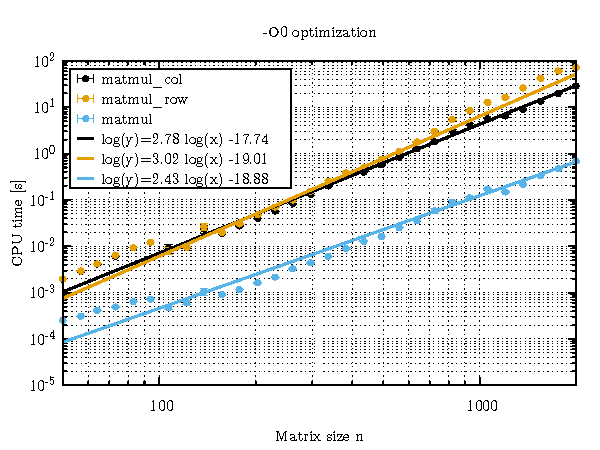
\includegraphics[width=0.5\textwidth]{images/flag-O0.pdf}
	\caption{\label{fig:04_R_1} Performances of the two implementations and of the intrinsic function depending on the matrix size \( n \), without using optimization flags.}
\end{figure}

Moreover, the performances of the algorithms are analyzed for different optimization flags added at compile time, such as \code{-O1}, \code{-O2}, \code{-O3} and \code{-Ofast}. For these cases, the results are showed respectively in Figures \ref{fig:04_R_2}, \ref{fig:04_R_3}, \ref{fig:04_R_4} and \ref{fig:04_R_5}.
Lastly, every result for the slope coefficient obtained by fit is reported in Table \ref{tab:04_R_12345} along with the associated uncertainty.

\begin{figure*}[!h]
    \centering
    \subfloat[][{\small \codebold[black]{-O1}}]{
        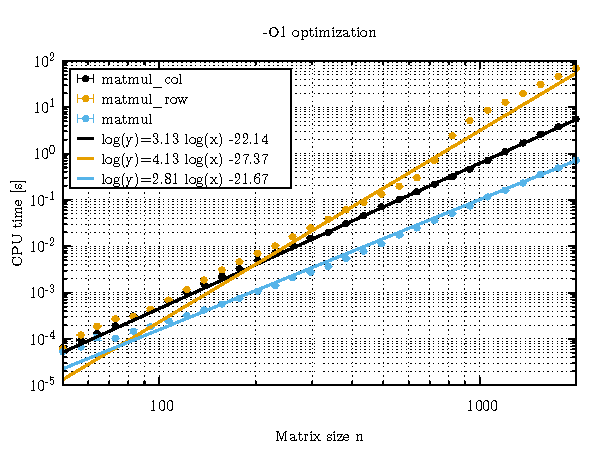
\includegraphics[width=0.48\textwidth]{images/flag-O1.pdf}
        \label{fig:04_R_2}
    }
    \hfill
    \subfloat[][{\small \codebold[black]{-O2}}]{
        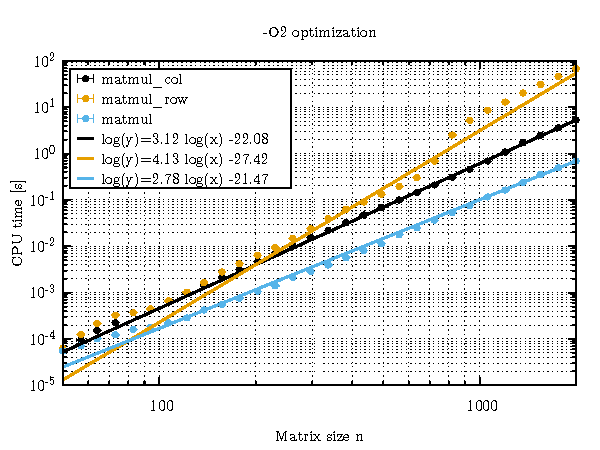
\includegraphics[width=0.48\textwidth]{images/flag-O2.pdf}
        \label{fig:04_R_3}
    }

    \subfloat[][{\small \codebold[black]{-O3}}]{
        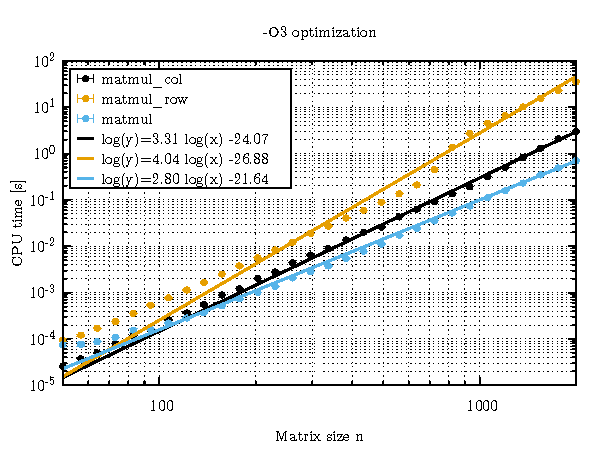
\includegraphics[width=0.48\textwidth]{images/flag-O3.pdf}
        \label{fig:04_R_4}
    }
    \hfill
    \subfloat[][{\small \codebold[black]{-Ofast}}]{
        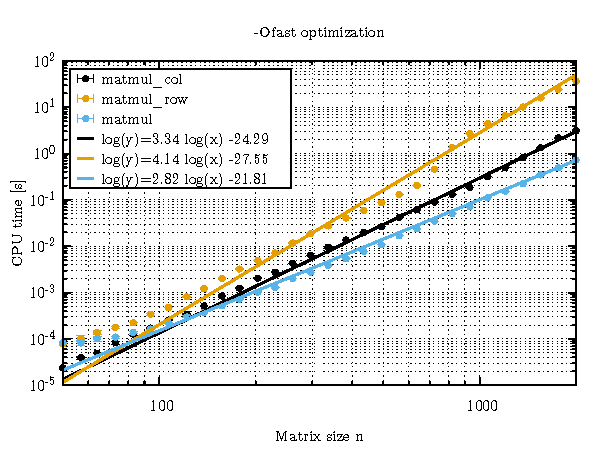
\includegraphics[width=0.48\textwidth]{images/flag-Ofast.pdf}
        \label{fig:04_R_5}
    }
    \caption{Comparison of performances depending on \( n \) for different optimization flags.}
    \label{fig:04_R_2345}
\end{figure*}

As we can see from the plot without optimization flags (\code{-O0}), the results for \code{matmul\_row} is in agreement with an expected slope coefficient of \( \sim 3 \), showing however some fluctuations. The slope for \code{matmul\_col} and, in particular, for the intrinsic \code{matmul} are significantly smaller, due to a more efficient implementation.

Concerning the cases with optimization flags, we can see from the plots how the results change, showing a deviation from the expected slope for \code{matmul\_row}. Insted, \code{matmul\_col} still agrees with the expectation, while \code{matmul} shows worse results with respect to the case of no optimization flags but still below the complexity of \( \mathcal{O}(n^{3}) \).

\begin{table}[!h]
    \begin{tabular}{|c|c|c|c|}
        \toprule
        \textbf{Flag}   &   \( \mathbf{m}_{\codebold[black]{matmul\_col}} \ \si{[s^{-1}]}\)  &   \( \mathbf{m}_{\codebold[black]{matmul\_row}} \ \si{[s^{-1}]}\)  &   \( \mathbf{m}_{\codebold[black]{MATMUL}} \ \si{[s^{-1}]}\)   \\
        \colrule
        \codebold[black]{-O0}      &   \( 2.78 \pm 0.05 \)   &   \( 3.02 \pm 0.08 \) &   \( 2.43 \pm 0.05 \)   \\
        \codebold[black]{-O1}      &   \( 3.14 \pm 0.02 \)   &   \( 4.1 \pm 0.2 \)   &   \( 2.81 \pm 0.03 \)   \\
        \codebold[black]{-O2}      &   \( 3.12 \pm 0.03 \)   &   \( 4.1 \pm 0.2 \)   &   \( 2.78 \pm 0.03 \)   \\
        \codebold[black]{-O3}      &   \( 3.31 \pm 0.04 \)   &   \( 4.0 \pm 0.2 \)   &   \( 2.80 \pm 0.03 \)   \\
        \codebold[black]{-Ofast}   &   \( 3.34 \pm 0.05 \)   &   \( 4.1 \pm 0.2 \)   &   \( 2.83 \pm 0.03 \)   \\
        \botrule
    \end{tabular}
    \caption{Slope coefficients for every case, obtained from fit results.}
    \label{tab:04_R_12345}
\end{table}





\section{Self-evaluation}
The implementation of the code has led to interesting results. Deviations from the expected behaviour are found for both implementations in different cases. These observations require further studies, possibly scanning larger values of \( n \), in order to find a valid explanation. However, this cannot actually be done because of the insufficient computational power of the machine on which the code is executed.
\end{document}
